%%%%%%%%%%%%%%%%%%%%%%%%%%%%%%%%%%%%%%%%%%%%%%%
%
% Template per Elaborato di Laurea
% DISI - Dipartimento di Ingegneria e Scienza dell’Informazione
%
% update 2015-09-10
%
% Per la generazione corretta del 
% pdflatex nome_file.tex
% bibtex nome_file.aux
% pdflatex nome_file.tex
% pdflatex nome_file.tex
%
%%%%%%%%%%%%%%%%%%%%%%%%%%%%%%%%%%%%%%%%%%%%%%%

% formato FRONTE RETRO
\documentclass[epsfig,a4paper,11pt,titlepage,twoside,openany]{book}
\usepackage{epsfig}
\usepackage{plain}
\usepackage{setspace}
\usepackage[paperheight=29.7cm,paperwidth=21cm,outer=1.5cm,inner=2.5cm,top=2cm,bottom=2cm]{geometry} % per definizione layout
\usepackage{titlesec} % per formato custom dei titoli dei capitoli
\usepackage{url}
\usepackage{graphicx}
\usepackage{mathtools}
\usepackage{tabularx, ragged2e}


%%%%%%%%%%%%%%
% supporto lettere accentate
%
%\usepackage[latin1]{inputenc} % per Windows;
\usepackage[utf8x]{inputenc} % per Linux (richiede il pacchetto unicode);
%\usepackage[applemac]{inputenc} % per Mac.

\singlespacing

\usepackage[english]{babel}

\begin{document}

  % nessuna numerazione
  \pagenumbering{gobble} 
  \pagestyle{plain}

\thispagestyle{empty}

\begin{center}
  \begin{figure}[h!]
    \centerline{
\psfig{file=logo_unitn_black_center.eps,width=0.6\textwidth}}
  \end{figure}

  \vspace{2 cm} 

  \LARGE{Department of Information Engineering And Computer Science\\}

  \vspace{1 cm} 
  \Large{Bachelor degree in\\
    Computer Science
    %Ingegneria dell'Informazione e delle Comunicazioni
    %Ingegneria dell'Informazione e Organizzazione d'Impresa
    %Ingegneria Elettronica e delle Telecomunicazioni
  }

  \vspace{2 cm} 
  \Large\textsc{Final Dissertation\\} 
  \vspace{1 cm} 
  \Huge\textsc{Integration of Bitcoin Cash in R\\}
  \Large{\it{Sottotitolo (alcune volte lungo - opzionale)}}


  \vspace{2 cm} 
  \begin{tabular*}{\textwidth}{ c @{\extracolsep{\fill}} c }
  \Large{Supervisor} & \Large{Candidate/Student}\\
  \Large{Agostinelli Claudio}& \Large{Vasile Adrian Bogdan Pop}\\
  \end{tabular*}

  \vspace{2 cm} 

  \Large{Accademic Year 2018/2019}
  
\end{center}



  \clearpage
 
%%%%%%%%%%%%%%%%%%%%%%%%%%%%%%%%%%%%%%%%%%%%%%%%%%%%%%%%%%%%%%%%%%%%%%%%%%
%%%%%%%%%%%%%%%%%%%%%%%%%%%%%%%%%%%%%%%%%%%%%%%%%%%%%%%%%%%%%%%%%%%%%%%%%%
%% Nota
%%%%%%%%%%%%%%%%%%%%%%%%%%%%%%%%%%%%%%%%%%%%%%%%%%%%%%%%%%%%%%%%%%%%%%%%%%
%% Sezione Ringraziamenti opzionale
%%%%%%%%%%%%%%%%%%%%%%%%%%%%%%%%%%%%%%%%%%%%%%%%%%%%%%%%%%%%%%%%%%%%%%%%%%
%%%%%%%%%%%%%%%%%%%%%%%%%%%%%%%%%%%%%%%%%%%%%%%%%%%%%%%%%%%%%%%%%%%%%%%%%%
  \thispagestyle{empty}

\begin{center}
  {\bf \Huge Ringraziamenti}
\end{center}

\vspace{4cm}


\emph{
  ...thanks to...
}

  \clearpage
  \pagestyle{plain} % nessuna intestazione e pie pagina con numero al centro

  
  % inizio numerazione pagine in numeri arabi
  \mainmatter

%%%%%%%%%%%%%%%%%%%%%%%%%%%%%%%%%%%%%%%%%%%%%%%%%%%%%%%%%%%%%%%%%%%%%%%%%%
%%%%%%%%%%%%%%%%%%%%%%%%%%%%%%%%%%%%%%%%%%%%%%%%%%%%%%%%%%%%%%%%%%%%%%%%%%
%% Nota
%%%%%%%%%%%%%%%%%%%%%%%%%%%%%%%%%%%%%%%%%%%%%%%%%%%%%%%%%%%%%%%%%%%%%%%%%%
%% Si ricorda che il numero massimo di facciate e' 30.
%% Nel conteggio delle facciate sono incluse 
%%   indice
%%   sommario
%%   capitoli
%% Dal conteggio delle facciate sono escluse
%%   frontespizio
%%   ringraziamenti
%%   allegati    
%%%%%%%%%%%%%%%%%%%%%%%%%%%%%%%%%%%%%%%%%%%%%%%%%%%%%%%%%%%%%%%%%%%%%%%%%%
%%%%%%%%%%%%%%%%%%%%%%%%%%%%%%%%%%%%%%%%%%%%%%%%%%%%%%%%%%%%%%%%%%%%%%%%%%

    % indice
    \tableofcontents
    \clearpage


    \chapter*{Abstract} % senza numerazione
\label{abstract}

\addcontentsline{toc}{chapter}{Abstract} % da aggiungere comunque all'indice

The thesis attempts to explain what a blockchain is, 
how it works and why it seems to have so much potential. 
In particular, this debate focuses on the different purposes of this
technology with its functionalities and its implementations by 
analysing two specific blockchains: Bitcoin (BTC)\cite{bitcoin.org} and Bitcoin Cash (BCH)\cite{bitcoincash}. 
The thesis also exposes which are the requirements 
a blockchain should have when it is used as a coin, in order to be 
globally handled as the leading currency. Hence, it goes deeper into the
differences between the BTC and BCH analysing the distinct approaches to 
satisfy the demands of a cryptocurrency. Especially, it illustrates
the main reasons why the Bitcoin hard fork was reached on August 1st, 
2017, giving life to the Bitcoin Cash blockchain.
Once the behaviour of this new technology is clear, the thesis goes 
further with the integration of BCH in the programming language \textit{R} (see section \ref{sec:environment} for more details).
In this way, it provides a means to work with the data stored into the Bitcoin
Cash blockchain and retrieve interesting statistics regarding it.

  In other words, the steps to achieve the goal for this thesis will be:



\begin{itemize}
  \item Understanding and analysing blockchain technologies.
  \item Studying the two most important Bitcoin blockchains: BTC - Bitcoin and BCH - Bitcoin Cash.
  \item Designing a new Package in R for data reading and manipulation of the Bitcoin Cash blockchain.
  \item Implementation of the Package in R with a description of all the possible commands developed.
  \item Example of the Package functionalities and its potential.
\end{itemize}





    \clearpage
    
          
    % gruppo per definizone di successione capitoli senza interruzione di pagina
    \begingroup
      % nessuna interruzione di pagina tra capitoli
      % ridefinizione dei comandi di clear page
      \renewcommand{\cleardoublepage}{} 
      \renewcommand{\clearpage}{} 
      % redefinizione del formato del titolo del capitolo
      % da formato
      %   Capitolo X
      %   Titolo capitolo
      % a formato
      %   X   Titolo capitolo
      
      \titleformat{\chapter}
        {\normalfont\Huge\bfseries}{\thechapter}{1em}{}
        
      \titlespacing*{\chapter}{0pt}{0.59in}{0.02in}
      \titlespacing*{\section}{0pt}{0.20in}{0.02in}
      \titlespacing*{\subsection}{0pt}{0.10in}{0.02in}
      
      % sommario
      

%%%%%%%%%%%%%%%%%%%%%%%%%%%%%%%%%%%%%%%%%%%%%%%%%%%%%%%%%%%%%%%%%%%%%%%%%%
%%%%%%%%%%%%%%%%%%%%%%%%%%%%%%%%%%%%%%%%%%%%%%%%%%%%%%%%%%%%%%%%%%%%%%%%%%
%% Nota
%%%%%%%%%%%%%%%%%%%%%%%%%%%%%%%%%%%%%%%%%%%%%%%%%%%%%%%%%%%%%%%%%%%%%%%%%%
%% Sommario e' un breve riassunto del lavoro svolto dove si descrive 
%% l’obiettivo, l’oggetto della tesi, le metodologie e 
%% le tecniche usate, i dati elaborati e la spiegazione delle conclusioni 
%% alle quali siete arrivati.
%% Il sommario dell’elaborato consiste al massimo di 3 pagine e deve contenere le seguenti informazioni: 
%%   contesto e motivazioni
%%   breve riassunto del problema affrontato
%%   tecniche utilizzate e/o sviluppate
%%   risultati raggiunti, sottolineando il contributo personale del laureando/a
%%%%%%%%%%%%%%%%%%%%%%%%%%%%%%%%%%%%%%%%%%%%%%%%%%%%%%%%%%%%%%%%%%%%%%%%%%
%%%%%%%%%%%%%%%%%%%%%%%%%%%%%%%%%%%%%%%%%%%%%%%%%%%%%%%%%%%%%%%%%%%%%%%%%%      
      
      %%%%%%%%%%%%%%%%%%%%%%%%%%%%%%%%
      % lista dei capitoli
      %
      % \input oppure \include
      %
      \chapter{Blockchain}
\label{cha:blockchain}

The application of the blockchain in multiple fields is gaining more and more 
traction today to the point of which some are even considering it the new Internet\cite{newinternet}.
But actually, the main concept behind this revolutionary idea was described as 
early as 1991 in an academic paper\cite{haber}
published by Stuart Haver and W. Scott Stornetta. With their solution, the two 
scientists aimed to Time-Stamp documents, in order to certify when a document
was created or last changed. The system used a cryptographically secured 
chain of blocks to store the time-stamped documents and in 1992 Merkle 
trees\cite{merkletree} were incorporated into the design, making it more efficient by 
allowing several documents to be collected into one block.\cite{binancevision}
However, this was not enough. Indeed, in order to have a fully working blockchain 
more components are needed.




\section{Distributed ledger}
\label{sec:ledger}

As said in a report from the UK Government, "A distributed ledger is 
essentially an asset database that can be shared across a network of 
multiple sites, geographies or institutions. All participants within a 
network can have their own identical copy of the ledger"\cite{ukgov}.
Due to this technology, there are neither central administrators nor 
centralized data storages. To have this mechanism working, both
a Peer-to-Peer Network (the peers are computer systems connected
to each other via the Internet, the data can be shared directly between 
systems on the network) and a Consensus Algorithm are needed(See section \ref{sec:consensus} for more details). 

\begin{figure}[h]
    \centering
    
\includegraphics[height=5cm, width=\textwidth]{distributed.png}
    \caption{Representation of the different types of network architecture.\cite{fauna}}
    \label{fig:dis}
\end{figure}

\section{Consensus Algorithms}
\label{sec:consensus}

To clarify the benefits of this type of algorithm we must start with a 
dilemma known as "The Byzantine Generals Problem"\cite{byzantine}, in which, each 
general has its own army and each group is situated in different 
locations around the city they intend to attack. The generals need to 
agree on either attacking or retreating. It does not matter whether 
they attack or retreat, as long as all generals reach consensus, 
i.e., agree on a common decision in order to execute it in coordination. 
Therefore, the following requirements are to be considered:
\begin{itemize}
    \item Each general has to decide: attack or retreat (yes or no).
    \item After the decision is made, it cannot be changed.
    \item All generals have to agree on the same decision and execute it in a synchronized manner.
\end{itemize}
The aforementioned communication problems are related to the fact that 
one general is only able to communicate with another through messages, 
which are forwarded by a courier. Consequently, the central challenge 
of the Byzantine Generals’ Problem is that the messages can get somehow 
delayed, destroyed or lost.

Further, even if a message is successfully delivered, one or more 
generals may choose (for whatever reason) to act maliciously and send 
a fraudulent message to confuse the other generals, leading to a total 
failure.

If we apply the dilemma to the context of blockchains, each general 
represents a network node, and the nodes need to reach consensus on 
the current state of the system. To clarify the concept, the majority 
of participants within a distributed network have to agree and execute 
the same action to avoid complete failure.\cite{byzantine}\cite{binancevision}
There are various implementations of the mechanism through which a blockchain 
network may reach consensus.


\subsection{Proof of Work}
\label{sec:pow}

Due to Bitcoin (see \ref{cha:bitcoin} for more details), the most known consensus algorithm is the Proof of 
Work (PoW), in which is employed for block generation. 
The process of generating correct proofs to add a block 
to the blockchain is known as “mining” and the individuals that 
participate in the mining process are known as “miners”.\cite{consensusmedium}

PoW mining involves numerous hashing attempts, so more computational 
power means more trials per second. In other words, miners with a high 
hash rate have better chances to find a valid solution for the next 
block. The PoW consensus algorithm makes sure that miners are only able 
to validate a new block and add it to the blockchain as long as 
the distributed nodes of the network reach consensus and agree that the 
block hash provided by the miner is a valid proof of work.\cite{binancevision}

\subsection{Proof of Stake}
\label{sec:pos}

The Proof of Stake (PoS) consensus algorithm 
is relatively different and a new way to generate and append blocks in a 
blockchain. It was developed in 2011 as an alternative to PoW, which requires
a massive amount of energy to make it work. In fact, according to the 
bitcoin energy consumption tracker at Digiconomist\cite{digiconomist}, 
bitcoin currently consumes 66.7 terawatt-hours per year. That is comparable 
to the total energy consumption of the Czech Republic, a country 
of 10.6 million people.

\begin{figure}[h]
    \centering
    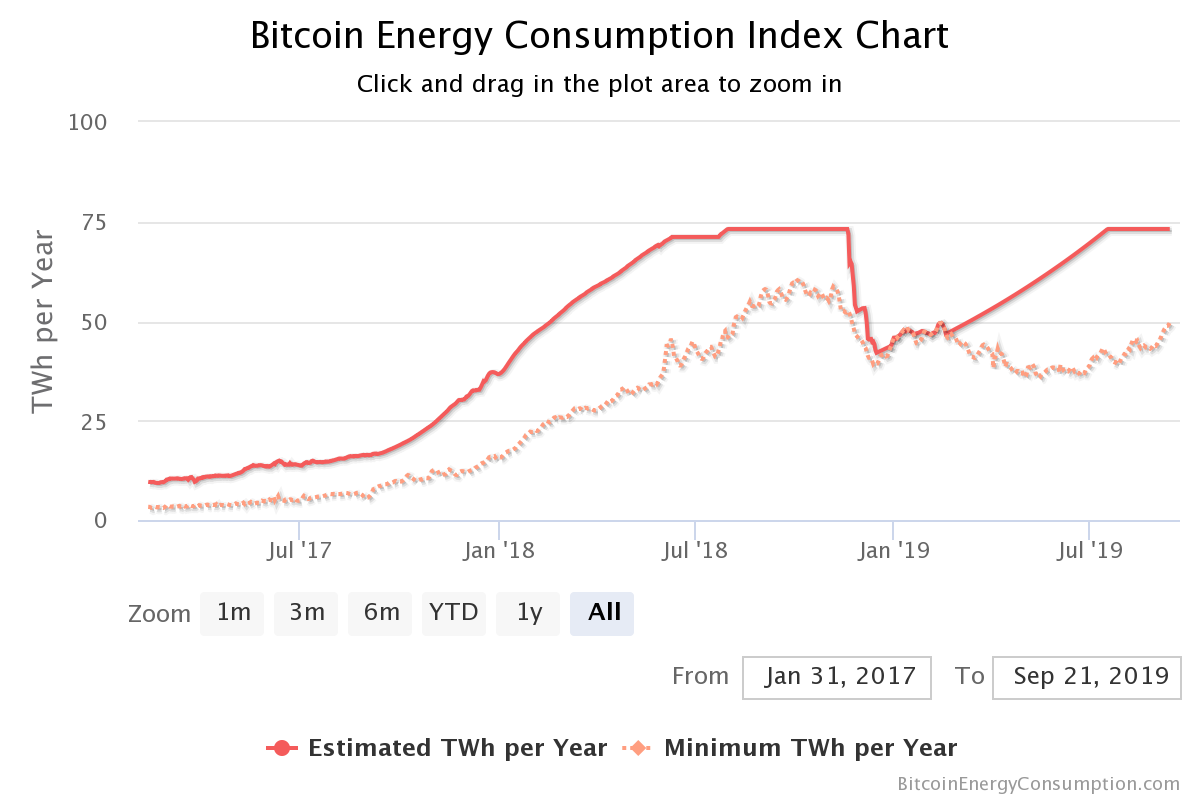
\includegraphics[height=7cm]{energy.png}
    \caption{Bitcoin energy consumption in the mining process.\cite{digiconomist}}
    \label{fig:energy}
\end{figure}

Basically, the mining process is replaced with a mechanism where blocks are
validated according to the stake of the participants, also known as "validators".
The criteria used to choose the validator depends on the proof of stake system
but mainly, the choice is based on the economic stake in the network of 
each node.\cite{binancevision}\cite{consensusmedium}

\subsection{Proof of Burn}
\label{sec:pob}

The Proof of Burn (PoB) algorithm is an approach to avoid the massive 
waste of energy used for hashing. Indeed, with this technique, the mining
process is replaced with a greener one. Where, the "miners" of the PoB 
coins will send coins to an  unspendable address, known as "eater address".
Even these transactions are recorded on the blockchain ensuring that the coin 
cannot be spent again. The principle behind this consensus algorithm is that
the user burning the cryptocurrency is showing long-term commitment to the
coin by burning it. This is because they are taking a short-term loss in 
exchange for a long-term gain.\cite{consensusmedium}




\section{Advantages and Disadvantages}
\label{sec:evaluate}

As a result of its complexity, blockchain's potential as a distributed 
form of record-keeping is almost without limit. But like every other 
technology, even the blockchain has its pros and cons. 

\subsection{Advantages}
\label{sec:advantages}

\textbf{Trustless system and small fees.}
In most traditional systems, a consumer pays a bank to verify a transaction,   
a notary to sign a document, or a minister to perform a marriage. Using 
blockchain technologies, this is no longer necessary because the distributed
nodes verify the transactions through consensus algorithms.\\
Therefore, blockchain systems negate the risk of trusting a single person or 
organization and reduces the overall costs and transaction fees by cutting 
third-parties. For this reason, blockchain is often referred to as a "trustless"
system.\cite{binancevision}\cite{investopedia}\bigskip\\ 
%\textbf{Improved accuracy by removing human involvement in verification.} 
%\bigskip\\
\textbf{Transactions are secure, private and efficient.}
By eliminating the human factor, we obtain a 24 hour a day 
working system, instead of institutions operating only during business hours.
As a result, transactions can be completed in about ten minutes and can be 
considered secure after just a few hours. Actually, once a transaction is 
recorded, its authenticity must be verified by the blockchain network where 
millions of nodes rush to confirm that the details of the transaction are correct.

Moreover, every block of the chain has the hash of the block before it along with
its own hash, which is computed with the data contained in the block. So, when
a piece of information in a block is edited in any way, its own hash will change, but the
hash in the block after it will not. This contrast makes it extremely difficult to 
change data inside the blockchain without being noticed.

\begin{figure}[h]
    \centering
    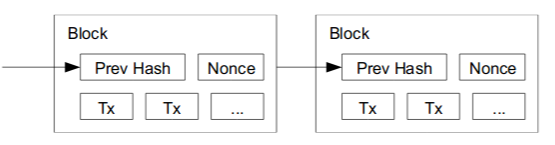
\includegraphics[height=4cm]{block_hash.png}
    \caption{A sample of the chain of blocks.\cite{bitcoin}}
    \label{fig:blockhash}
\end{figure}

Considering that the majority of blockchains are public, means that anyone 
can access the blockchain and read the data inside it with all the transaction 
history. So, if anyone can read all the transactions, why do people say that
blockchain transactions are anonymous?\\
This is because anonymity is confused with confidentiality. Indeed, every user makes 
public transactions with their unique code called "public key",
which is recorded on the blockchain, rather than their personal information.\cite{investopedia}
"Public key cryptography" is a cryptographic system that uses pairs of keys: public keys which may 
be disseminated widely, and private keys which are known only to the owner.\pagebreak

\textbf{Transparency.}
A big benefit to this technology is given by its open-source nature. This means
that the users of the blockchain network can modify the code as they consider is the most fitting for their purposes, so long
as they have the approval from the majority of the network's nodes.\bigskip\\

\textbf{Distributed.}
Blockchain does not store any of its information in a unique node or central 
location. Instead, data is stored in thousands of devices on a distributed
network. Whenever a block is added to the chain, every node updates its blockchain
to reflect the change. Because of this, there is no single point of failure
and so it becomes more difficult to tamper with.\cite{binancevision}\cite{investopedia}\bigskip\\

\textbf{Stability.}
Once a block is confirmed, it is extremely difficult to remove or change the data inside it.
This makes blockchain a great technology for storing financial records or any other data 
where an audit trail is required because every change is tracked and permanently recorded 
on a distributed and public ledger.\cite{binancevision}
\bigskip

\subsection{Disadvantages}
\label{sec:disadvantages}

While there are significant benefits to the blockchain, there are also serious
challenges to its adoption. The most signigivatives ones are political and regulatory\cite{investopedia}, but 
there are also some technical challenges to take into account.\bigskip\\

\textbf{Private keys.} 
Blockchain uses public key cryptography to give users ownership over their blockchain data.
Each public key corresponds to a private key which should be kept secret. Users need their 
private key to access their data. If a user loses its private key, the money is 
effectively lost, and there is nothing they can do about it.\cite{binancevision}\\

\begin{figure}[h]
    \centering
    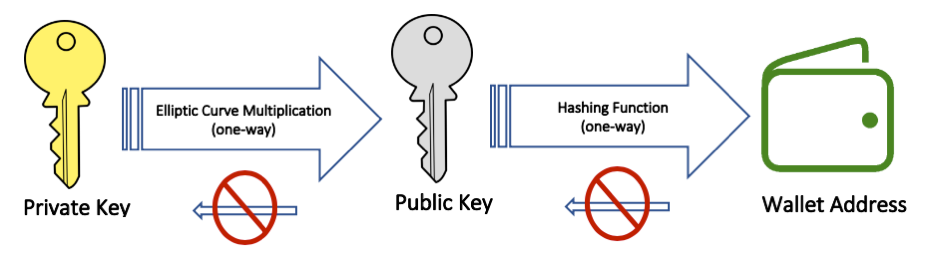
\includegraphics[height=4.3cm]{key_generation.png}
    \caption{Private key, public key, and address generation flow.\cite{key}}
    \label{fig:key}
\end{figure}\bigskip
\textbf{Energy inefficiency.}
Some blockchains, especially those using Proof of Work consensus algorithms \ref{sec:pow}, are 
highly inefficient. Since mining is highly competitive and there is 
only one winner every ten minutes, the work of every other miner is wasted.
As miners are continously trying to increase their computational power 
to have a greater chance of finding a valid block hash, the resources used 
by the Bitcoin network increased significantly in the last few years, and it 
currently consumes more energy than that of many countries, such as Denmark, Ireland, 
and Nigeria.\cite{binancevision}
\bigskip 
\textbf{Scalability.}
The Bitcoin is a perfect case study for the low scalability of blockchains.
In fact, to add a new block on the blockchain, it takes about ten minutes and
the maximum size of each block is of 1 MegaBytes. This entails that there is a
limited number of transactions per block. It is estimated that Bitcoin's 
blockchain can manage only seven transactions per second (TPS). Meanwhile, the
Visa's actual infrastructure can process 24.000 TPS.\cite{investopedia}\pagebreak
\bigskip 
\textbf{51\% Attacks.}
The consensus algorithms that protect the blockchain have proven to be very 
efficient over the years (thanks to Bitcoin). However, there are a few potential attacks that can 
be performed against blockchain networks. The most discussed is the  51\% attack.
Such an attack may happen if one entity manages to control more than 50\% of the 
network, which would allow them to edit or modify the order of the transactions.
Although it is theoretically possible, there has never been a successful 51\% attack on 
the Bitcoin blockchain, additionally, as the network gets larger, the security 
increases.\cite{binancevision}
\bigskip 
\textbf{Storage.}
Distributed ledgers can increase significantly over time. For example, the Bitcoin blockchain
currently requires 239 GigaByte of storage (Last update: 10/9/2019). Even if in 
the Bitcoin paper it is said that thanks to "Moore's Law"\cite{bitcoin} the storage should
not be a problem, the current growth in blockchain size appears to be outstripping the growth
in hard drives and at the same time the network risks losing nodes if the ledger becomes too large for 
individuals to download and store.\cite{binancevision}


\section{Use Cases}
\label{sec:usecases}

The merit to the great attention given to the blockchain technology is to be attributed
to Bitcoin. Indeed, thanks to these digital currencies (cryptocurrencies) the 
blockchain-based solutions have grown. So learning how this innovative technology
can be applied to different scenarios is very important. 

\subsection{Digital Identity}
\label{sec:identity}

The identity component in a blockchain is fulfilled through the use of cryptographic keys.
Combining a public and private key creates a strong digital identity reference based 
on possession of pieces of information or certifications. The public key is distributed 
publicly and it is what identifies the identity, whereas the private key is kept secret by
the identity and it is used to express consent to digital interactions and to 
sign the data to record in the block.\cite{coindesk}

To make an example, it could be useful when one has to prove some information 
about themselves. Suppose someone has a digital copy of the driver's license 
and then that person must prove to be old enough to drink. The bartender could verify
the proof using the public key of the issuer. But the bartender never learns his
actual birth date, that is what it is called "Zero Knowledge Proof".\cite{sovrin}

\begin{figure}[h]
    \centering
    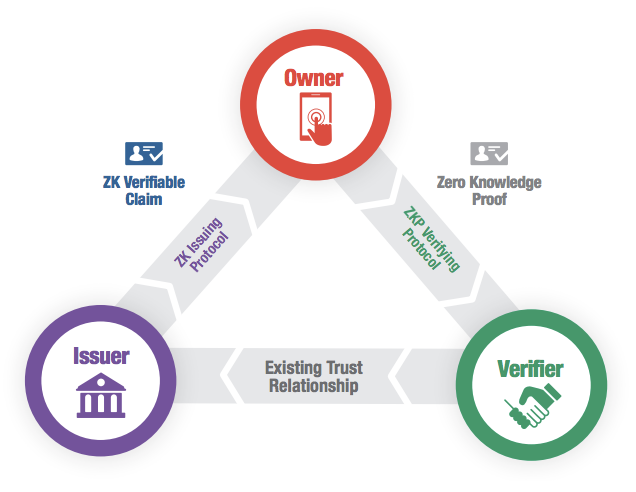
\includegraphics[height=7cm]{identity.png}
    \caption{Zero Knowledge Verifiable Claims.\cite{sovrin}}
    \label{fig:claim}
\end{figure}\pagebreak

\subsection{Charity}
\label{sec:charity}

The number of charitable organizations which are adopting cryptocurrencies as a donation
method is increasing more and more. The reason is due to crypto's transparency,
in fact, thanks to this characteristic, every donation can be tracked and verified.
So, the higher is the level of transparency and public accountability, the easier will be for donors  
to be encouraged to make an offer and as a consequence the charity’s 
reputation for integrity will be reinforced too.
Moreover, blockchain technology reduces fees and taxes to manage every donation by
reducing the number of required intermediaries.\cite{binancevision}

\begin{figure}[h]
    \centering
    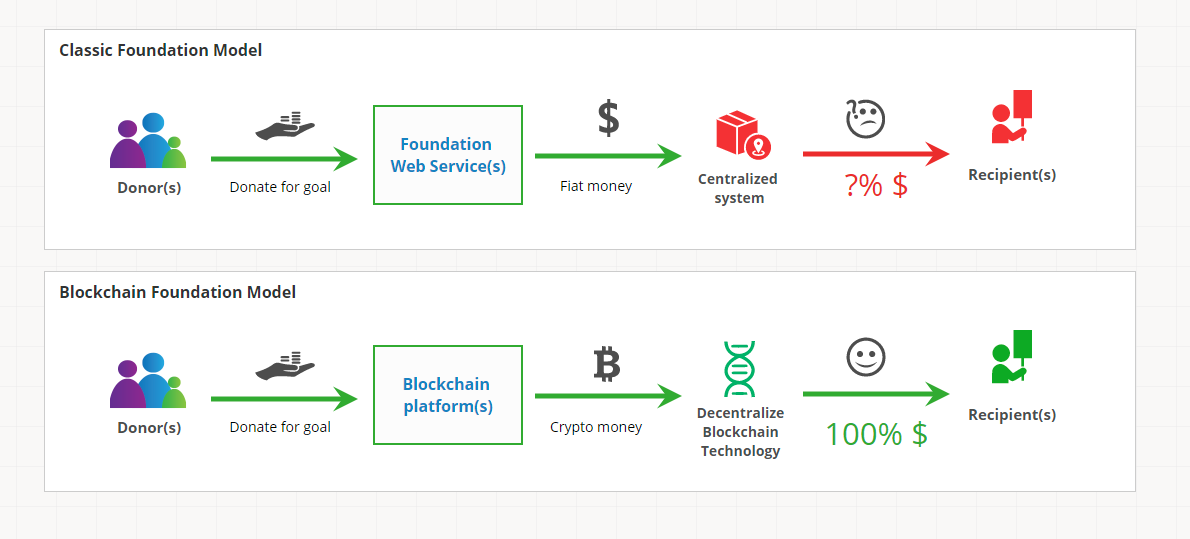
\includegraphics[height=5cm]{charity.png}
    \caption{Charity donation schema.\cite{cointelegraph}}
    \label{fig:donation}
\end{figure}

\subsection{Healthcare}
\label{sec:healthcare}

Blockchain may offer significant benefits to hospitals in terms of security, 
interoperability, and transparency. Unlike traditional databases that rely on a centralized
server, the use of a distributed system allows for data exchange with higher levels of 
security. In addition, distributed ledgers increase the interoperability among clinics,
hospitals, and other health service providers by allowing all of these parties to interface
with a unique storage system.

Furthermore, blockchain systems may also give higher levels of accessibility and 
transparency over their own health information. But also, allow pharmaceutical 
organizations to increase the efficiency of their infrastructure by cutting 
down on the widespread problem of drug counterfeiting.\cite{binancevision}

\subsection{Governance}
\label{sec:governance}

Governance can be greatly improved in various sectors by blockchain technologies.
A short example can be the efficiency of taxes, given that governments rely on 
taxpayer funds, they must use their budgets wisely. Blockchain systems 
and smart contracts can be employed to automate tasks and workflows, which would 
greatly reduce time and money spent on bureaucratic processes.\cite{binancevision}

Another application can be the election process. With the support of a working digital 
identity system and the high level of immutability given by the blockchain, this 
technology could be an excellent solution for ensuring that votes cannot be tampered with.
Creating the possibility to transform the secure online voting into a reality. 

\subsection{Payments}
\label{sec:payments}

Thanks to Bitcoin, this is the most widespread application of the blockchain. It started in 
2008 when Satoshi Nakamoto published the Bitcoin's white paper, where, for the first time, 
all the above components of a blockchain were used to solve the double-spending problem.\pagebreak



      \chapter{Bitcoin}
\label{cha:bitcoin}

In a few words, Bitcoin is a digital form of actual cash. But in unlike the 
traditional fiat currency, which relies on a central bank controlling it, this new
form of currency relies on blockchain technology and cryptography. 
In computer science, "cryptography" refers to secure information and communication 
techniques derived from mathematical concepts and a set of rule-based calculations 
called algorithms to transform messages in ways that are hard to decipher.
As a result, this new digital cash is mainly referred to as ''cryptocurrency''.

\section{Infrastructure}
\label{sec:Infrastructure}

Bitcoin, as the majority of cryptos, is based on a public permissionless blockchain architecture.
Which means that anyone can join, read, write and commit, plus it is hosted on public 
servers, is anonymous and is highly resilient. \\
The Bitcoin's mechanism to reach consensus is the Proof of Work algorithm \ref{sec:pow}.
Due to the implementation described by Satoshi Nakamoto in the white paper "The proof-of-work 
involves scanning for a value that when hashed, such as with SHA-256, the hash begins 
with a number of zero bits. The average work required is exponential in the number of 
zero bits required and can be verified by executing a single hash. For our timestamp 
network, we implement the proof-of-work by incrementing a \textit{nonce} (a 32-bit value of the block)\ in the block until a 
value is found that gives the block's hash the required zero bits.   
Once the CPU effort   has   been   expended   to   make   it   satisfy   the   
proof-of-work,   the   block   cannot   be   changed without  redoing  the   work.    
As   later   blocks   are  chained   after  it,   the  work  to  change  the  
block would include redoing all the blocks after it"\cite{bitcoin}. It follows 
that the difficulty required to close a block is flexible. In fact, it changes every 
2016 blocks suiting the computational power of the network. Considering that, at the 
desired rate of one block every 10 minutes, 2016
blocks mean that the difficulty is adjusted every two weeks.

\subsection{Incentive}
\label{sec:incentive}

To have a working PoW, miners have to spend their CPU time and electricity. So, why 
should they allocate their resources in Bitcoin?

The answer is the incentive. Indeed, the first transaction of every block is a special
transaction which gives a new amount of currency to the creator of the block. This, 
not only is a good incentive to support the network but also provides a way to initially 
distribute coins into circulation, since there is no central authority to issue them.
\begin{figure}[!h]
    \centering
    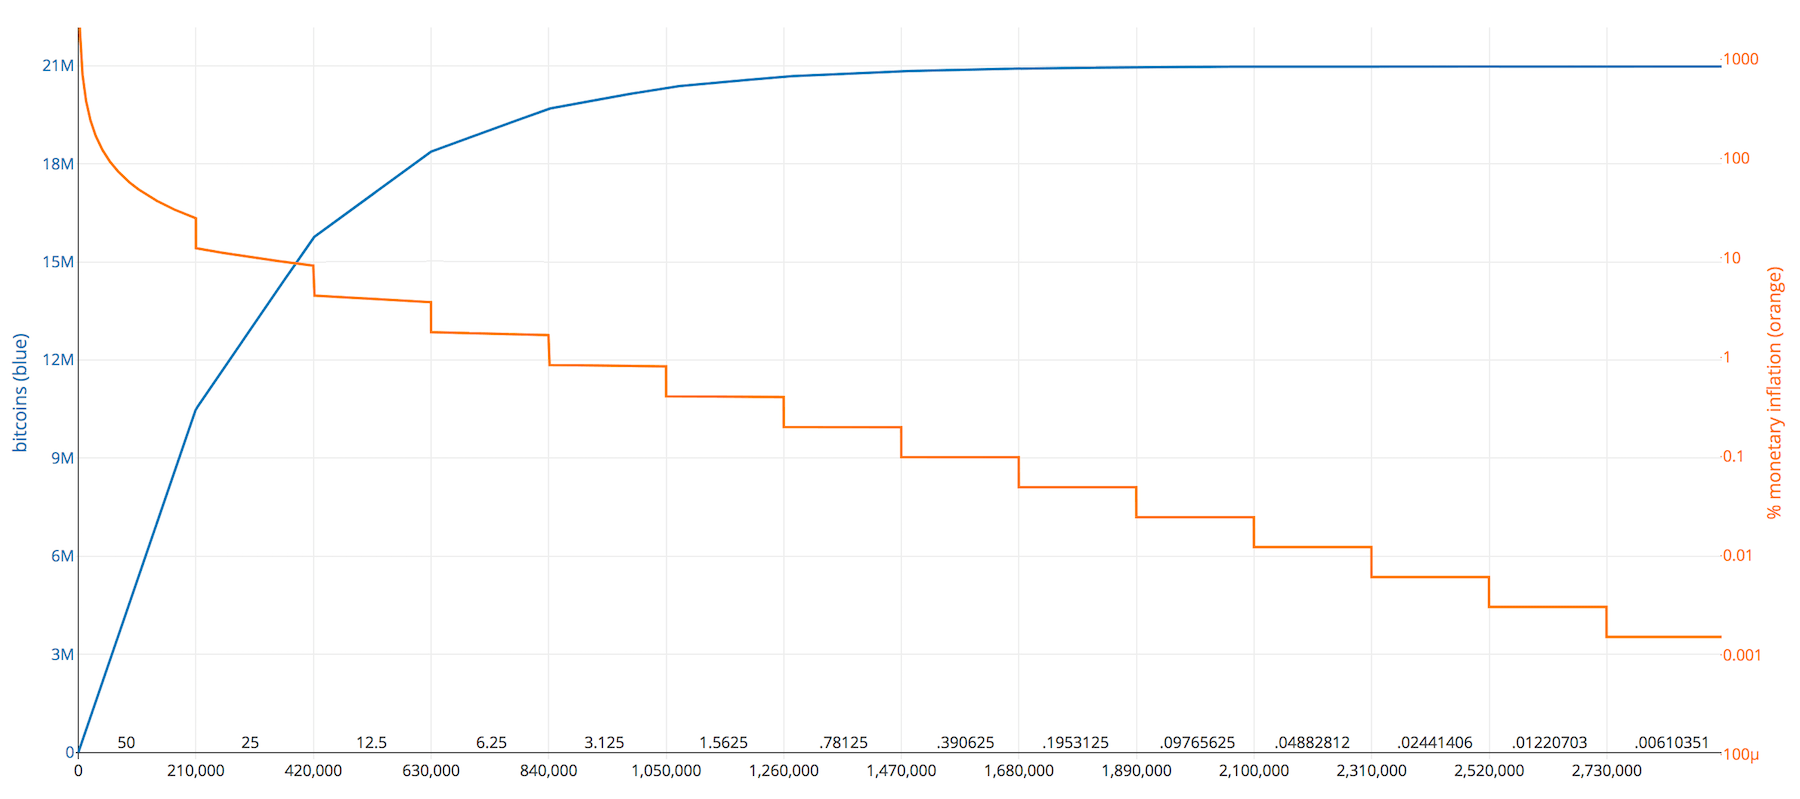
\includegraphics[width = 0.8\textwidth]{rewarding.png}
    \caption{How mining rewarding is planned over time.\cite{rewarding}}
    \label{fig:claim}
\end{figure} 
However, this process is destinated to end, because there is a predetermined number
of coins (21 million) which can spread. To ensure that, every 210.000 blocks 
(corresponding to 4 years), the reward given to the creator of the block is halved.
This leads to the second type of incentive in the Bitcoin network: transaction fees.
In fact, for every transaction, there is also a fee amount, which is given to the 
creator of the block as a reward for its effort.




\section{Transactions}
\label{sec:transactions}

To figure out how a transaction works, it is necessary to first understand the concept of
"owning a bitcoin". Because, unlike the fiat currency, where you own a physical coin
to spend, owning a bitcoin means that you own the key to unlock the coins from a past
transaction and use them in the new transaction. It is possible to get a better sense of the 
transaction mechanism, from a brief extract of the Bitcoin paper: 

"We define an electronic coin as a chain of digital signatures.  Each owner transfers 
the coin to the next by digitally signing a hash of the previous transaction and the 
public key of the next owner and adding these to the end of the coin.  A payee can 
verify the signatures to verify the chain of ownership"\cite{bitcoin}
\begin{figure}[h]
    \centering
    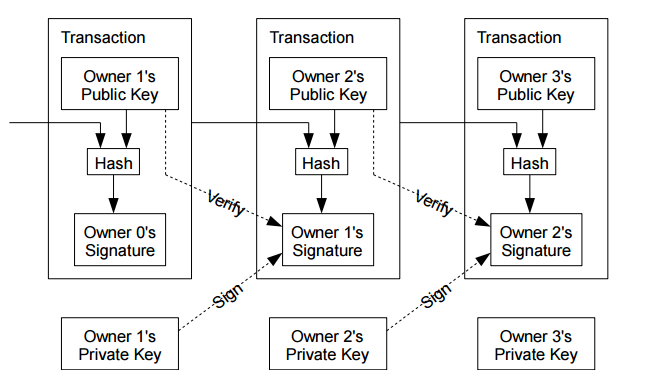
\includegraphics[height=6cm]{bitcoin-transaction.png}
    \caption{Transaction schema. From \cite{bitcoin}}
    \label{fig:trx}
\end{figure}

To go deeper into the design of a transaction, it is useful to imagine a double-entry
ledger. In a few words, every transaction has one or more "inputs" and one or more "outputs"
which are respectively debits and credits against a bitcoin address. 
Usually, outputs add up to slightly less than inputs, because the difference
represents an implicit "transaction fee" \ref{sec:incentive}. The higher the fee, the higher the 
probability for the transaction to be included in the next block to mine.

Each output, before it is spent as an input in a new transaction, waits as an "Unspent
Transaction Output" (UTXO). The sum of all the owned UTXOs, compose the total balance
of a wallet \ref{sec:wallets}.\\
But, not every transaction in the blockchain produces an UTXO.\\ 
It depends on the \textit{scriptPubKey} used in the specific transaction.
A scriptPubKey is ascript included in outputs which set the conditions that 
must be fulfilled for those satoshis to be spent. Data for fulfilling the conditions 
can be provided in a signature script (another type of data generated by the spender).
\bigskip 

\textbf{Pay To Public Key Hash (P2PKH)} 
Is the most common form of scriptPubKey used to send a transaction to one or multiple 
addresses. In this type of scriptPubKey, the coins sent can be unlocked by a single 
private key corresponding to the public key hashed in the transaction itself. It is 
possible to recognize it by looking at the first character in the address used for the
output. In fact, if it starts with the number "1" it is P2PKH.\cite{bitcoin.org}\pagebreak
\bigskip 

\textbf{Pay To Script Hash (P2SH)}
Was implemented in 2012 to add more flexibility to transactions by adding a hash 
of a second script, the redeem script. That is similar in function to a 
scriptPubKey. Where, one copy of it is hashed to create a P2SH address (used in an actual 
scriptPubKey) and another copy is placed in the spending signature script to enforce 
its conditions. It can be used to process multisignature transactions, 
Open Assets Protocol\footnote{Used to create new currencies upon the Bitcoin blockchain. 
Called colored coins} and to store textual data on the blockchain. The P2SH can 
be recognized by the number "3" at the begin of the addresses.\cite{bitcoin.org}\\

\begin{figure}[h]
    \centering
    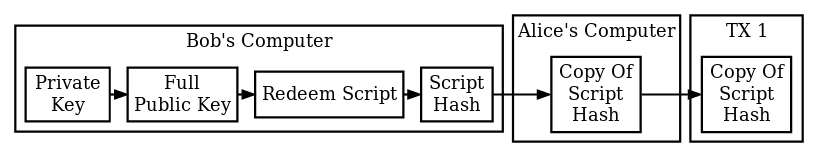
\includegraphics[width = 0.9\textwidth]{p2sh.png}
    \caption{creating A P2SH Redeem Script Hash To Receive Payments \cite{bitcoin.org}}
    \label{fig:p2sh}
\end{figure}\bigskip
\textbf{Multisig}
Are special addresses where to spend a transaction, the signature of multiple private keys are required.
Although P2SH multisig is now generally used for multisig transactions, this base 
script can be used to require multiple signatures before a UTXO can be spent.
In multisig pubkey scripts, called m-of-n, m is the minimum number of signatures 
which must match a public key; n is the number of public keys being provided.\cite{bitcoin.org}\\
\bigskip 

\textbf{Null Data}
This type adds arbitrary data to a probably unspendable scritptPubKey that nodes don't have
to store in their UTXOs database. Consensus rules allow null data outputs up to the maximum
allowed scriptPubKey size of 10.000 bytes provided.\cite{bitcoin.org}

\section{Wallets}
\label{sec:wallets}
In simple words, a wallet is the means through which is possible to manage all the 
owned cryptocurrency. But it can be split into two components, programs, and files.
Wallet programs create the public keys to receive the Bitcoin and use the 
corresponding private key to spend them.\\ 
Wallet files, instead, store the private keys in a file or physically on pieces of paper. 
Furthermore, it also provides both process used for the public-private key creation and 
usage, and approach to a deterministic hierarchy key creation process in an unlinkable
key manner.
\newpage



      \chapter{Bitcoin Cash}
\label{cha:bch}

"Imagine you have a dollar in your wallet, and you put it aside for a while and 
then realise that one coin has split in two. Sounds weird? Not in the cryptocurrency 
world." That is an analogy with the fiat currency reported in an article of 
Shouth China Morning Post\cite{scmp}.\\
Bitcoin is like a software, but, due to its distributed nature, unlike all the 
software we know, there isn't a single entity who determines how it should be 
updated. 

\section{Fork}
\label{sec:fork}

\subsection{SegWit}
\label{sec:segwit}

\subsection{Addresses}
\label{sec:addresses}

\subsection{Block Size}
\label{sec:blocksize}

\subsection{Block mining}
\label{sec:mining}

      \chapter{Package implementation in R}
\label{cha:R}

\section{Environment}
\label{sec:enivirionment}

\section{Feasibility study}
\label{sec:study}

\section{Implementation}
\label{sec:implementation}

\subsection{Commands}
\label{sec:blocksize}

\section{Usage samples}
\label{sec:mining}

      
      
    \endgroup


    % bibliografia in formato bibtex
    %
    % aggiunta del capitolo nell'indice
    \addcontentsline{toc}{chapter}{Bibliografia}
    % stile con ordinamento alfabetico in funzione degli autori
    \bibliographystyle{plain}
    \bibliography{biblio}
%%%%%%%%%%%%%%%%%%%%%%%%%%%%%%%%%%%%%%%%%%%%%%%%%%%%%%%%%%%%%%%%%%%%%%%%%%
%%%%%%%%%%%%%%%%%%%%%%%%%%%%%%%%%%%%%%%%%%%%%%%%%%%%%%%%%%%%%%%%%%%%%%%%%%
%% Nota
%%%%%%%%%%%%%%%%%%%%%%%%%%%%%%%%%%%%%%%%%%%%%%%%%%%%%%%%%%%%%%%%%%%%%%%%%%
%% Nella bibliografia devono essere riportati tutte le fonti consultate 
%% per lo svolgimento della tesi. La bibliografia deve essere redatta 
%% in ordine alfabetico sul cognome del primo autore. 
%% 
%% La forma della citazione bibliografica va inserita secondo la fonte utilizzata:
%% 
%% LIBRI
%% Cognome e iniziale del nome autore/autori, la data di edizione, titolo, casa editrice, eventuale numero dell’edizione. 
%% 
%% ARTICOLI DI RIVISTA
%% Cognome e iniziale del nome autore/autori, titolo articolo, titolo rivista, volume, numero, numero di pagine.
%% 
%% ARTICOLI DI CONFERENZA
%% Cognome e iniziale del nome autore/autori (anno), titolo articolo, titolo conferenza, luogo della conferenza (città e paese), date della conferenza, numero di pagine. 
%% 
%% SITOGRAFIA
%% La sitografia contiene un elenco di indirizzi Web consultati e disposti in ordine alfabetico. 
%% E’ necessario:
%%   Copiare la URL (l’indirizzo web) specifica della pagina consultata
%%   Se disponibile, indicare il cognome e nome dell’autore, il titolo ed eventuale sottotitolo del testo
%%   Se disponibile, inserire la data di ultima consultazione della risorsa (gg/mm/aaaa).    
%%%%%%%%%%%%%%%%%%%%%%%%%%%%%%%%%%%%%%%%%%%%%%%%%%%%%%%%%%%%%%%%%%%%%%%%%%
%%%%%%%%%%%%%%%%%%%%%%%%%%%%%%%%%%%%%%%%%%%%%%%%%%%%%%%%%%%%%%%%%%%%%%%%%%
    

    \titleformat{\chapter}
        {\normalfont\Huge\bfseries}{Allegato \thechapter}{1em}{}
    % sezione Allegati - opzionale
    \appendix
    %\chapter{Titolo primo allegato}

Lorem ipsum dolor sit amet, consectetur adipiscing elit. Donec sed nunc orci. Aliquam nec nisl vitae sapien pulvinar dictum quis non urna. Suspendisse at dui a erat aliquam vestibulum. Quisque ultrices pellentesque pellentesque. Pellentesque egestas quam sed blandit tempus. Sed congue nec risus posuere euismod. Maecenas ut lacus id mauris sagittis egestas a eu dui. Class aptent taciti sociosqu ad litora torquent per conubia nostra, per inceptos himenaeos. Pellentesque at ultrices tellus. Ut eu purus eget sem iaculis ultricies sed non lorem. Curabitur gravida dui eget ex vestibulum venenatis. Phasellus gravida tellus velit, non eleifend justo lobortis eget. 

\section{Titolo}
Lorem ipsum dolor sit amet, consectetur adipiscing elit. Donec sed nunc orci. Aliquam nec nisl vitae sapien pulvinar dictum quis non urna. Suspendisse at dui a erat aliquam vestibulum. Quisque ultrices pellentesque pellentesque. Pellentesque egestas quam sed blandit tempus. Sed congue nec risus posuere euismod. Maecenas ut lacus id mauris sagittis egestas a eu dui. Class aptent taciti sociosqu ad litora torquent per conubia nostra, per inceptos himenaeos. Pellentesque at ultrices tellus. Ut eu purus eget sem iaculis ultricies sed non lorem. Curabitur gravida dui eget ex vestibulum venenatis. Phasellus gravida tellus velit, non eleifend justo lobortis eget. 

\subsection{Sottotitolo}
Lorem ipsum dolor sit amet, consectetur adipiscing elit. Donec sed nunc orci. Aliquam nec nisl vitae sapien pulvinar dictum quis non urna. Suspendisse at dui a erat aliquam vestibulum. Quisque ultrices pellentesque pellentesque. Pellentesque egestas quam sed blandit tempus. Sed congue nec risus posuere euismod. Maecenas ut lacus id mauris sagittis egestas a eu dui. Class aptent taciti sociosqu ad litora torquent per conubia nostra, per inceptos himenaeos. Pellentesque at ultrices tellus. Ut eu purus eget sem iaculis ultricies sed non lorem. Curabitur gravida dui eget ex vestibulum venenatis. Phasellus gravida tellus velit, non eleifend justo lobortis eget. 


\chapter{Titolo secondo allegato}

Lorem ipsum dolor sit amet, consectetur adipiscing elit. Donec sed nunc orci. Aliquam nec nisl vitae sapien pulvinar dictum quis non urna. Suspendisse at dui a erat aliquam vestibulum. Quisque ultrices pellentesque pellentesque. Pellentesque egestas quam sed blandit tempus. Sed congue nec risus posuere euismod. Maecenas ut lacus id mauris sagittis egestas a eu dui. Class aptent taciti sociosqu ad litora torquent per conubia nostra, per inceptos himenaeos. Pellentesque at ultrices tellus. Ut eu purus eget sem iaculis ultricies sed non lorem. Curabitur gravida dui eget ex vestibulum venenatis. Phasellus gravida tellus velit, non eleifend justo lobortis eget. 

\section{Titolo}
Lorem ipsum dolor sit amet, consectetur adipiscing elit. Donec sed nunc orci. Aliquam nec nisl vitae sapien pulvinar dictum quis non urna. Suspendisse at dui a erat aliquam vestibulum. Quisque ultrices pellentesque pellentesque. Pellentesque egestas quam sed blandit tempus. Sed congue nec risus posuere euismod. Maecenas ut lacus id mauris sagittis egestas a eu dui. Class aptent taciti sociosqu ad litora torquent per conubia nostra, per inceptos himenaeos. Pellentesque at ultrices tellus. Ut eu purus eget sem iaculis ultricies sed non lorem. Curabitur gravida dui eget ex vestibulum venenatis. Phasellus gravida tellus velit, non eleifend justo lobortis eget. 

\subsection{Sottotitolo}
Lorem ipsum dolor sit amet, consectetur adipiscing elit. Donec sed nunc orci. Aliquam nec nisl vitae sapien pulvinar dictum quis non urna. Suspendisse at dui a erat aliquam vestibulum. Quisque ultrices pellentesque pellentesque. Pellentesque egestas quam sed blandit tempus. Sed congue nec risus posuere euismod. Maecenas ut lacus id mauris sagittis egestas a eu dui. Class aptent taciti sociosqu ad litora torquent per conubia nostra, per inceptos himenaeos. Pellentesque at ultrices tellus. Ut eu purus eget sem iaculis ultricies sed non lorem. Curabitur gravida dui eget ex vestibulum venenatis. Phasellus gravida tellus velit, non eleifend justo lobortis eget. 




\end{document}
